\documentclass{beamer}

\usepackage[pantone315,english]{wwustyle}

\usepackage[ngerman]{babel}
\usepackage[utf8]{inputenc}
\usepackage[T1]{fontenc}
\usepackage{multirow}
\usepackage{colortbl}
\usepackage{hhline}
\usepackage{subfigure} % Um mehrere Bilder in eine figure einzufügen

% Uncomment the following two lines if you want to prepare your document for
% the fast mode.
% \usetikzlibrary{external}
% \tikzexternalize

\author{Christof, Marvin, Sebastian, Pascal}
\title{RotEqNet}
%\institutelogo{Logo on title frame}
%\institutelogosmall{Logo on other frames}
\subtitle{Rotierte Kernel zur Bestimmung der Blickrichtung von Mistkäfern}

\begin{document}

%%%%%%%%%%%%%%% WWUstyle "fast" mode %%%%%%%%%%%%%%%%%%%%%
% Do the following steps in order to speed up the compilation time of your
% presentation:
%
% 1. Include the externalization tikz library in the preamble of your document.
%    This is always recommended if you are using tikz in your document.
% 2. Uncomment the \wwupreparefastmode command below
% 3. Compile your document with command line option '-shell-escape',
%    e.g.: 'pdflatex -shell-escape beamer.tex'
% 4. Comment (or delete) the \wwupreparefastmode
% 5. Add option 'fast' to the 'wwustyle' package declaration line.
% 6. Be happy!

% \wwupreparefastmode


\begin{frame}[plain]
  \maketitle
\end{frame}

\begin{frame}
	\frametitle{Gliederung}
	\begin{itemize}
		\item Motivation
		\item FIM - Datensatz
		\item Künstliche Neuronale Netze
		\item Metriken
		\item Autoencoder
		\item Deconvolution Neural Network
		\item Architekturen zur Bildsegmentierung
		\item Denoising Autoencoder
	\end{itemize}
\end{frame}

\begin{frame}
	\frametitle{Motivation}
	Bei RotEqNet (Rotation equivariant vector field network) handelt es sich um eine Convolutional-Netzarchitektur, welche sich durch folgende Punkte auszeichnet:
	\begin{itemize}
		\item zusätzliche Rotation der Kernel beim Bewegen über den Input
		\item sehr kompakte Modelle mit wenig Parametern
		\item vergleichbare Leistung zu Netzen mit deutlich größeren Modellen
		
	\end{itemize}
\end{frame}

\begin{frame}
	\frametitle{RotEqNet - Layers}
	\begin{block}{RotConv}
		\begin{itemize}
			\item[] \textbf{Forwardpass}
			\begin{itemize}
				\item Rotation eines kanonischen Grundfilters
				\item Anwendung der rotierten Filter auf den Input
				\item zusätzliche Durchpropagierung des Winkels
			\end{itemize}
			\item[] \textbf{Backwardpass}
			\begin{itemize}
				\item Rückrotation und Summation aller Gradienten
				\item Anpassung der Gewichte des kanonischen Filters
			\end{itemize}
		\end{itemize}
	\end{block}
\end{frame}

\begin{frame}
	\frametitle{RotEqNet - Layers}
	\begin{block}{Orientation Pooling}
		\begin{itemize}
			\item pixelweise Bestimmung der größten Magnitude
			\item Bestimmung des zugehörigen Winkels
			\item Anwendung von ReLu auf die Magnitude
			\item Umwandlung der Darstellung in kartesische Koordinaten
			\begin{itemize} 
				\item[$ \Rightarrow $] \normalsize Vectorfield
			\end{itemize}
		\end{itemize}
	\end{block}
\end{frame}

\begin{frame}
	\frametitle{RotEqNet - Layers}
	\begin{block}{Spatial Pooling}
			\begin{itemize}
				\item angepasste Version des Max-Pooling für Vectorfields
			\end{itemize}
	\end{block}
	\begin{block}{VectorBatchNorm}
		\begin{itemize}
			\item angepasste Version von BatchNorm für Vectorfields
			\item BatchNorm wird lediglich auf die Magnitude angewendet
		\end{itemize}
	\end{block}
\end{frame}

\begin{frame}
	\frametitle{Netzarchitektur}
	\footnotesize
	Für alle RotConv Layer gelten folgende Parameter:
	\begin{itemize}
		\item[] \textbf{Padding:} 9/2
		\item[] \textbf{R:} 17
	\end{itemize}
	\begin{minipage}[t]{0.5\linewidth}
		\begin{center}
			\footnotesize
		\begin{tabular}{|c|c|}
			\hline
			Layer & Parameter \\
			\hline \hline
			RotConv & (1, 4, [9x9])  \\
			Orientation Pooling &\\
			VectorBatchNorm & (4)\\
			Spatial Pooling & Factor: 2\\
			\hline	 
			RotConv & (4, 8, [9x9])  \\
			Orientation Pooling &\\
			VectorBatchNorm & (8)\\
			Spatial Pooling & Factor: 2\\
			\hline	
			RotConv & (8, 4, [9x9])  \\
			Orientation Pooling &\\
			VectorBatchNorm & (4)\\
			VectorUpsample & Factor: 2\\
			\hline	
			\end{tabular}
		\end{center}
	\end{minipage}%
	\begin{minipage}[t]{0.5\linewidth}
		\begin{center}
			\footnotesize
		\begin{tabular}{|c|c|}
			\hline
			RotConv & (4, 2, [9x9])  \\
			Orientation Pooling &\\
			VectorBatchNorm & (2)\\
			VectorUpsample & Factor: 2\\
			\hline
			RotConv & (2, 1, [9x9])  \\
			Orientation Pooling &\\
			\hline
			RotConv & (1, 1, [9x9])  \\
			Orientation Pooling &\\
			\hline
			Vector2Magnitude & \\
			\hline
		\end{tabular}
		\end{center}
\end{minipage}	
\end{frame}

\begin{frame}
	\frametitle{Entwicklung}
	Projekt geforked von Anders Waldeland
	\begin{itemize}
		\item Fix für Python 3 Kompatibilität
		\item Parser für .grndr Dateien
		\item Modularisierung des Codes und CleanUp
		\item Fix der mathematischen Berechnungen (nach Paper)
		\item Visualisierung des Vectorfields eines Bildes
		\item Training und Netzoptimierung anhand künstlichen Datensatzes
	\end{itemize}
\end{frame}

\begin{frame}
	\frametitle{Entwicklung}
	\begin{itemize}
		\item Test verschiedener Netzarchitekturen
		\begin{itemize}
			\item Object Detection (nur auf Magnitude)
			\item Klassifikation nach Winkeln
			\item komplettes Vectorfield (Magnitude und Winkel)
		\end{itemize}
		\item Test verschiedener Lossfunktionen
		\begin{itemize}
			\item BinaryCrossEntropy
			\item F1 Loss
			\item L1
			\item Smooth L1
			\item CategoricalCrossEntropy
		\end{itemize}
	\end{itemize}
\end{frame}

\begin{frame}
	\frametitle{Beispiel - Detection}
	\begin{minipage}{0.49\textwidth}
		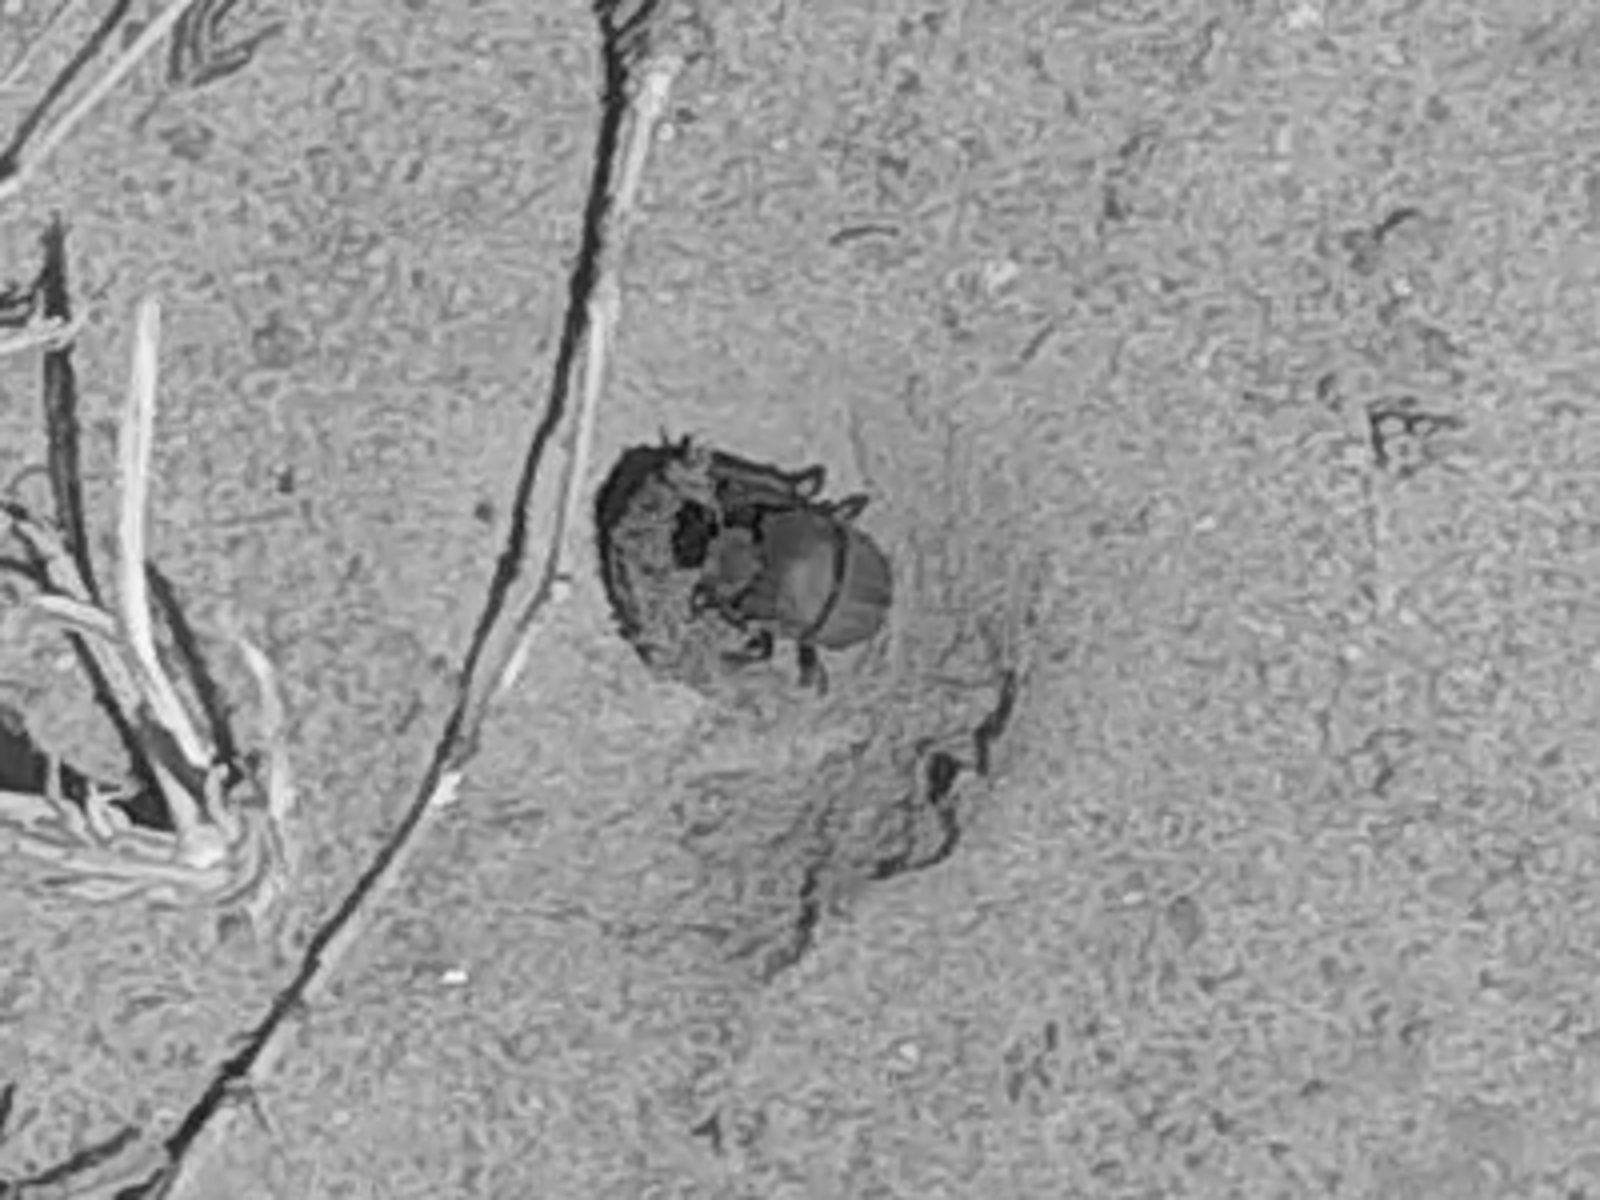
\includegraphics[width=\linewidth]{../Pictures/preferred_1_original.png}
	\end{minipage}
	\begin{minipage}{0.49\textwidth}
		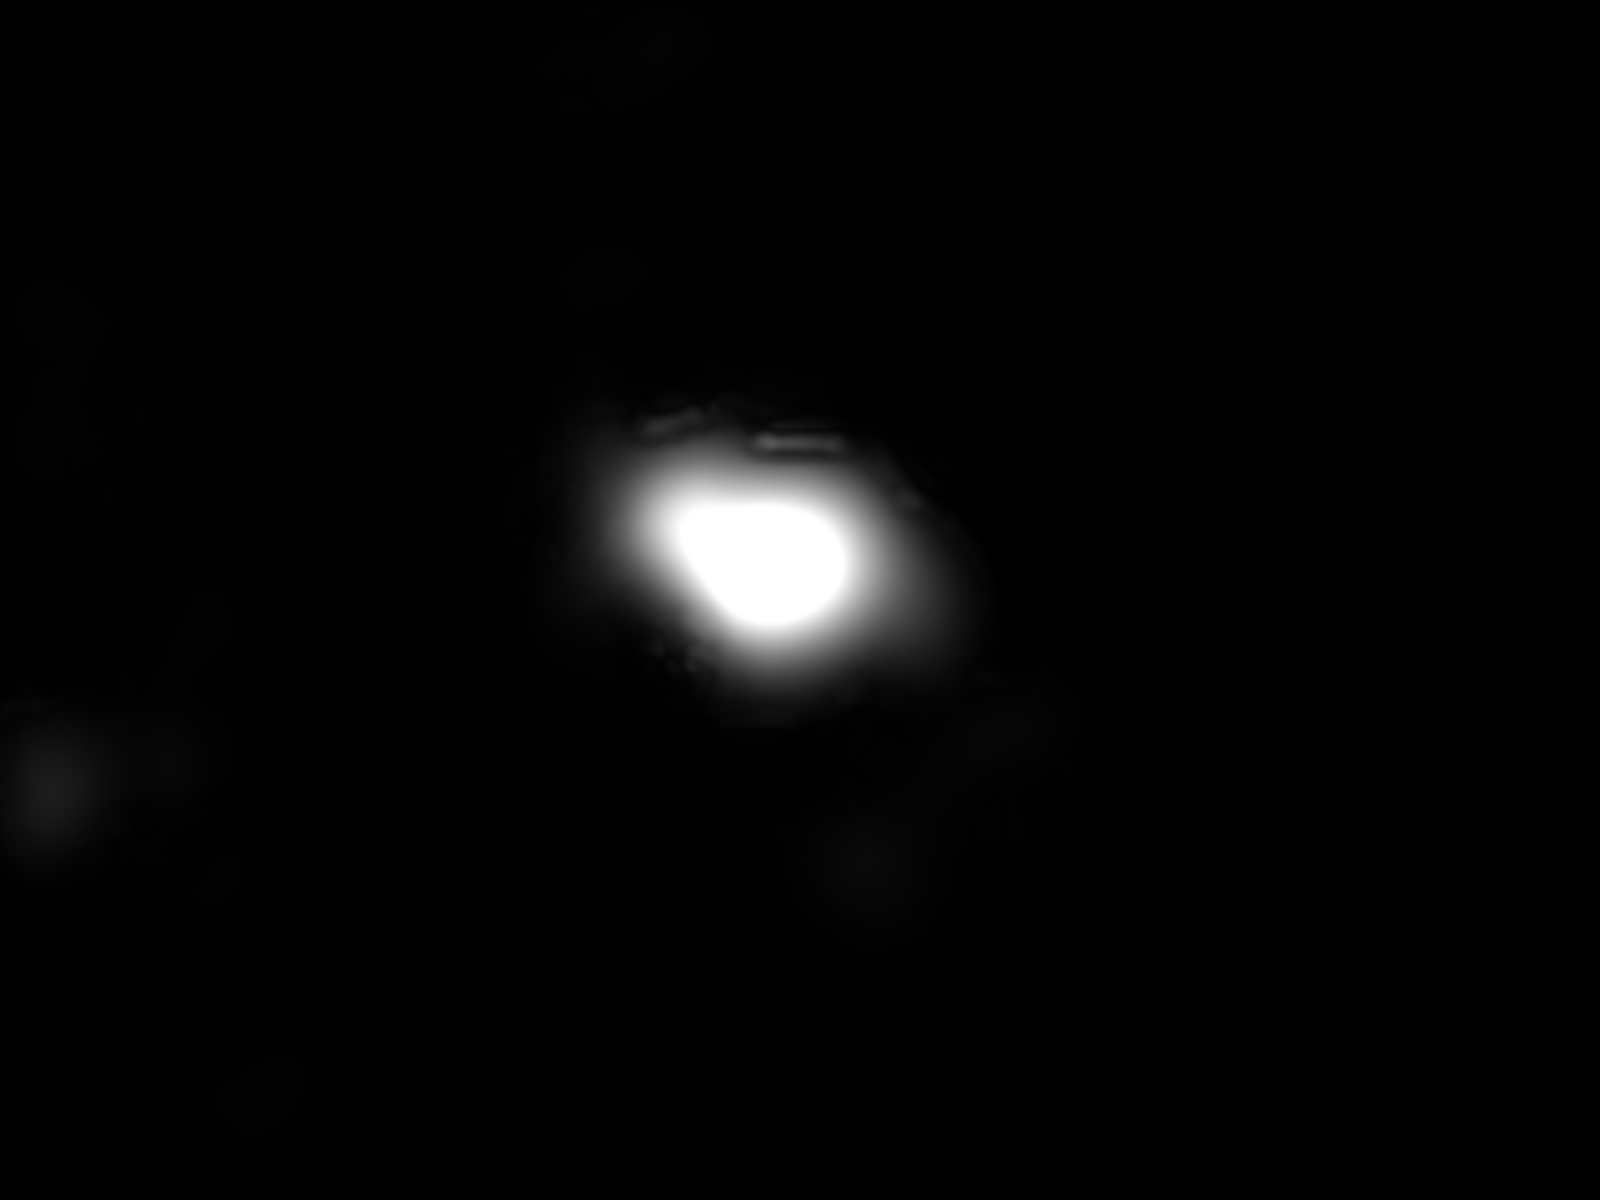
\includegraphics[width=\linewidth]{../Pictures/preferred_1_detection.png}
	\end{minipage}
\end{frame}

\begin{frame}
	\frametitle{Beispiel - Vectorfield}
	\begin{minipage}{0.49\textwidth}
		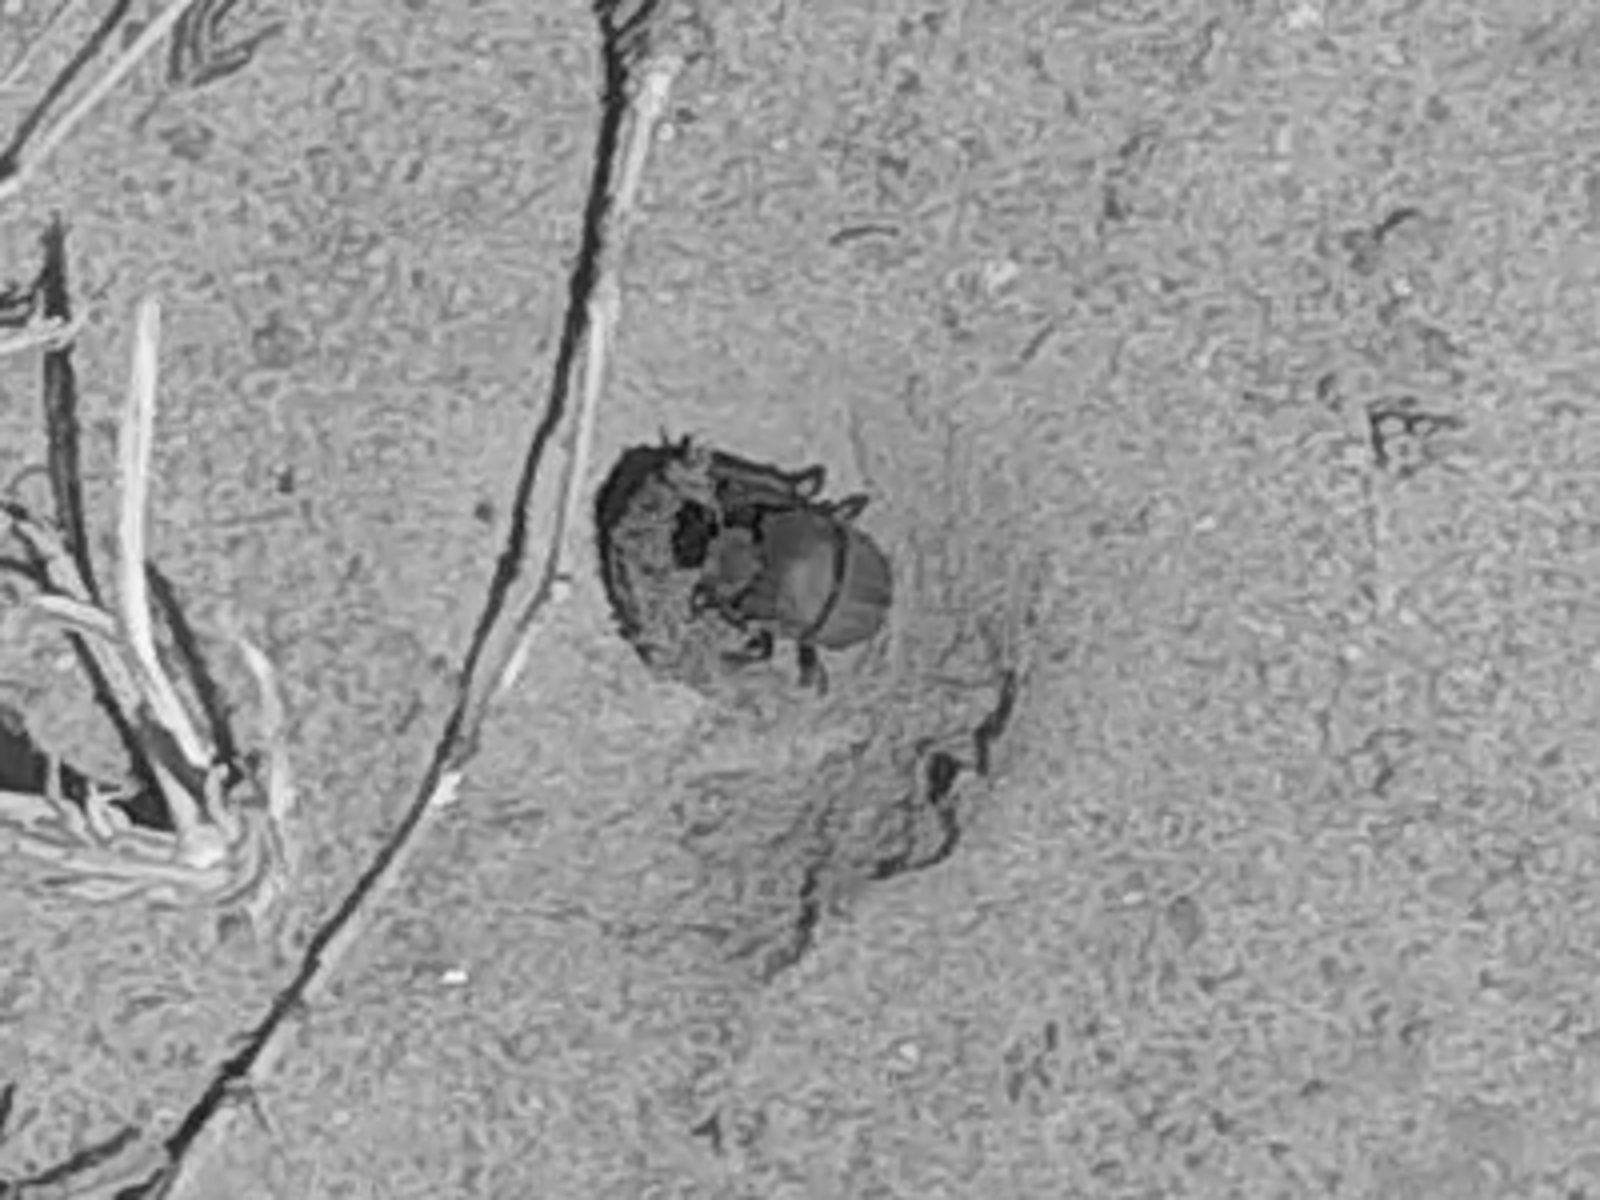
\includegraphics[width=\linewidth]{../Pictures/preferred_1_original.png}
	\end{minipage}
	\begin{minipage}{0.49\textwidth}
		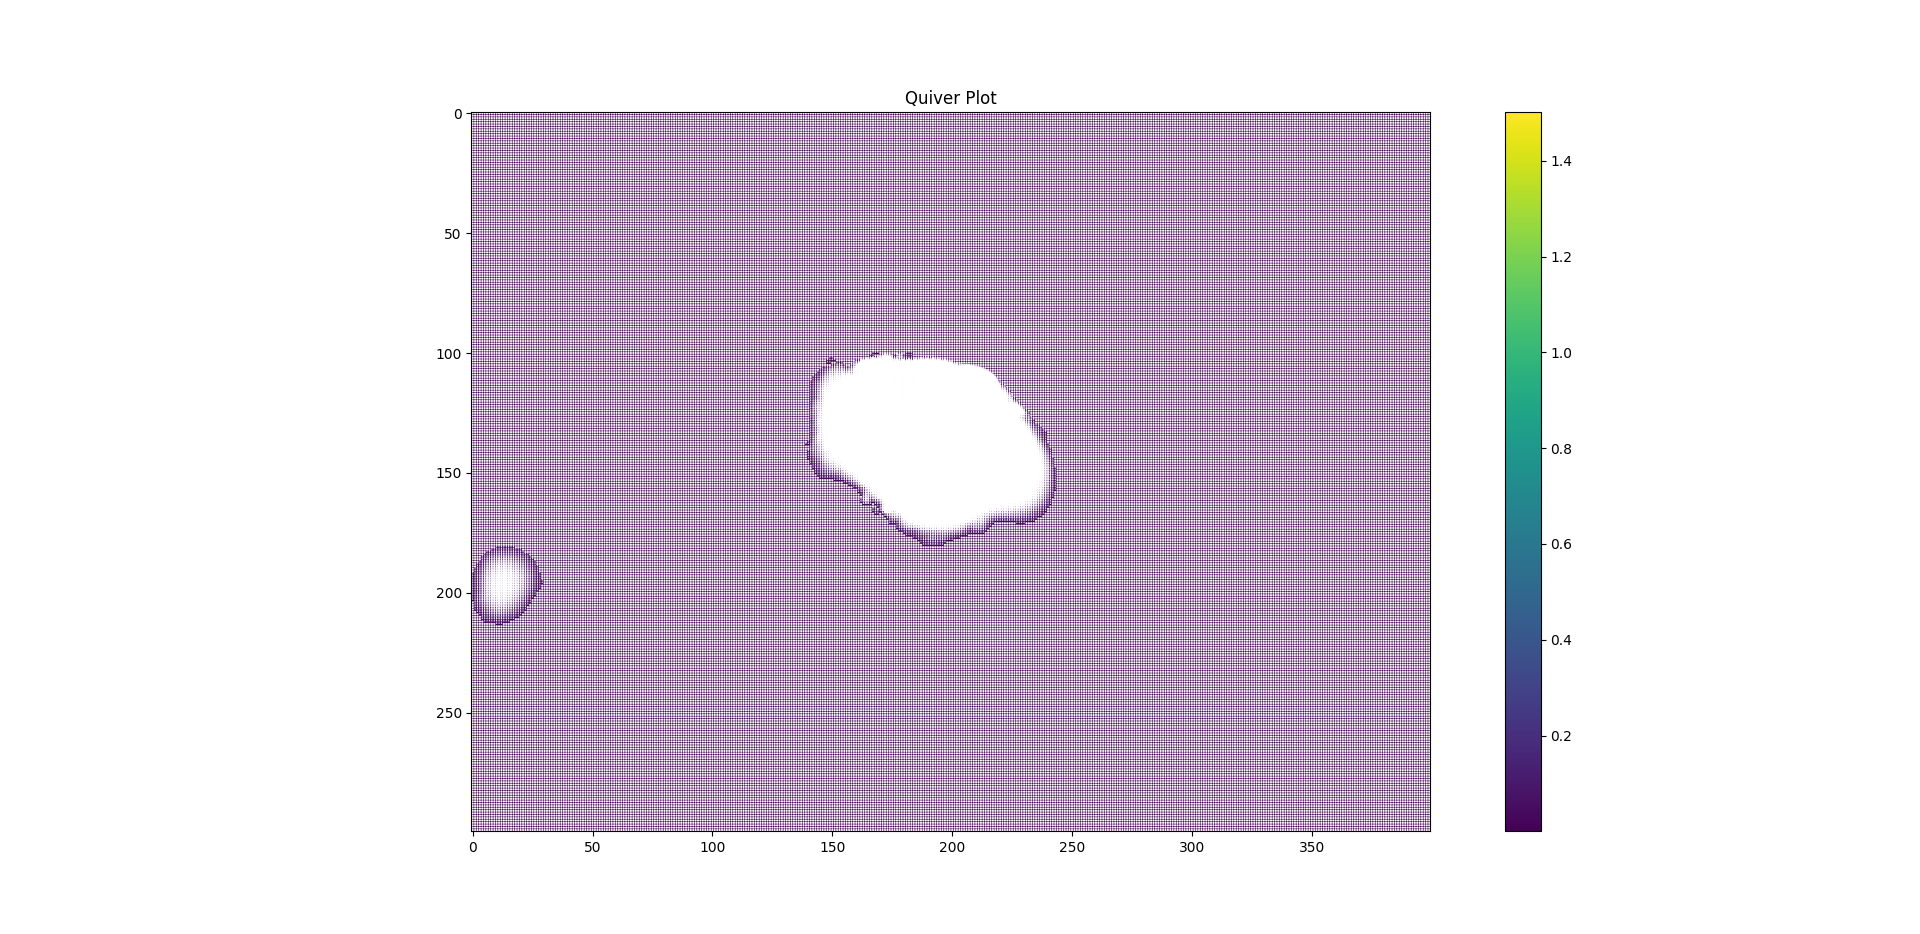
\includegraphics[width=\linewidth]{../Pictures/preferred_1_full.png}
	\end{minipage}
\end{frame}

\begin{frame}
	\frametitle{Beispiel - Vectorfield}
	\begin{minipage}{0.49\textwidth}
		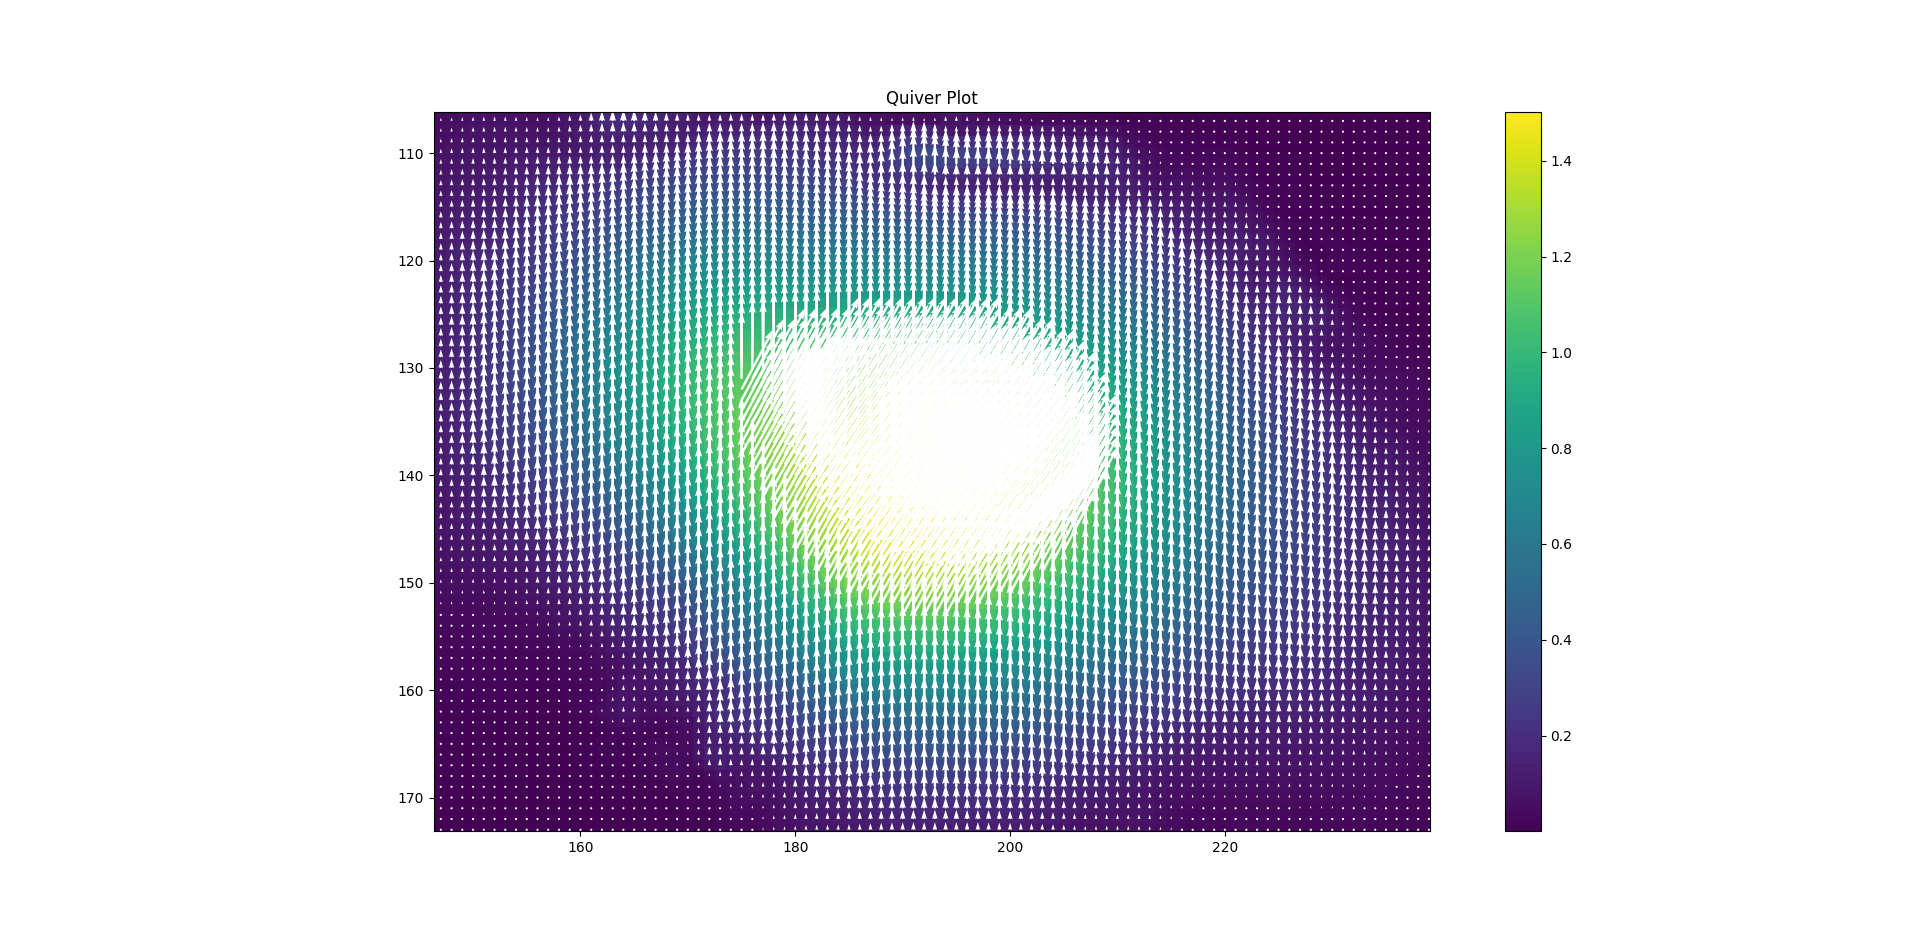
\includegraphics[width=\linewidth]{../Pictures/preferred_1_zoom.png}
	\end{minipage}
	\begin{minipage}{0.49\textwidth}
		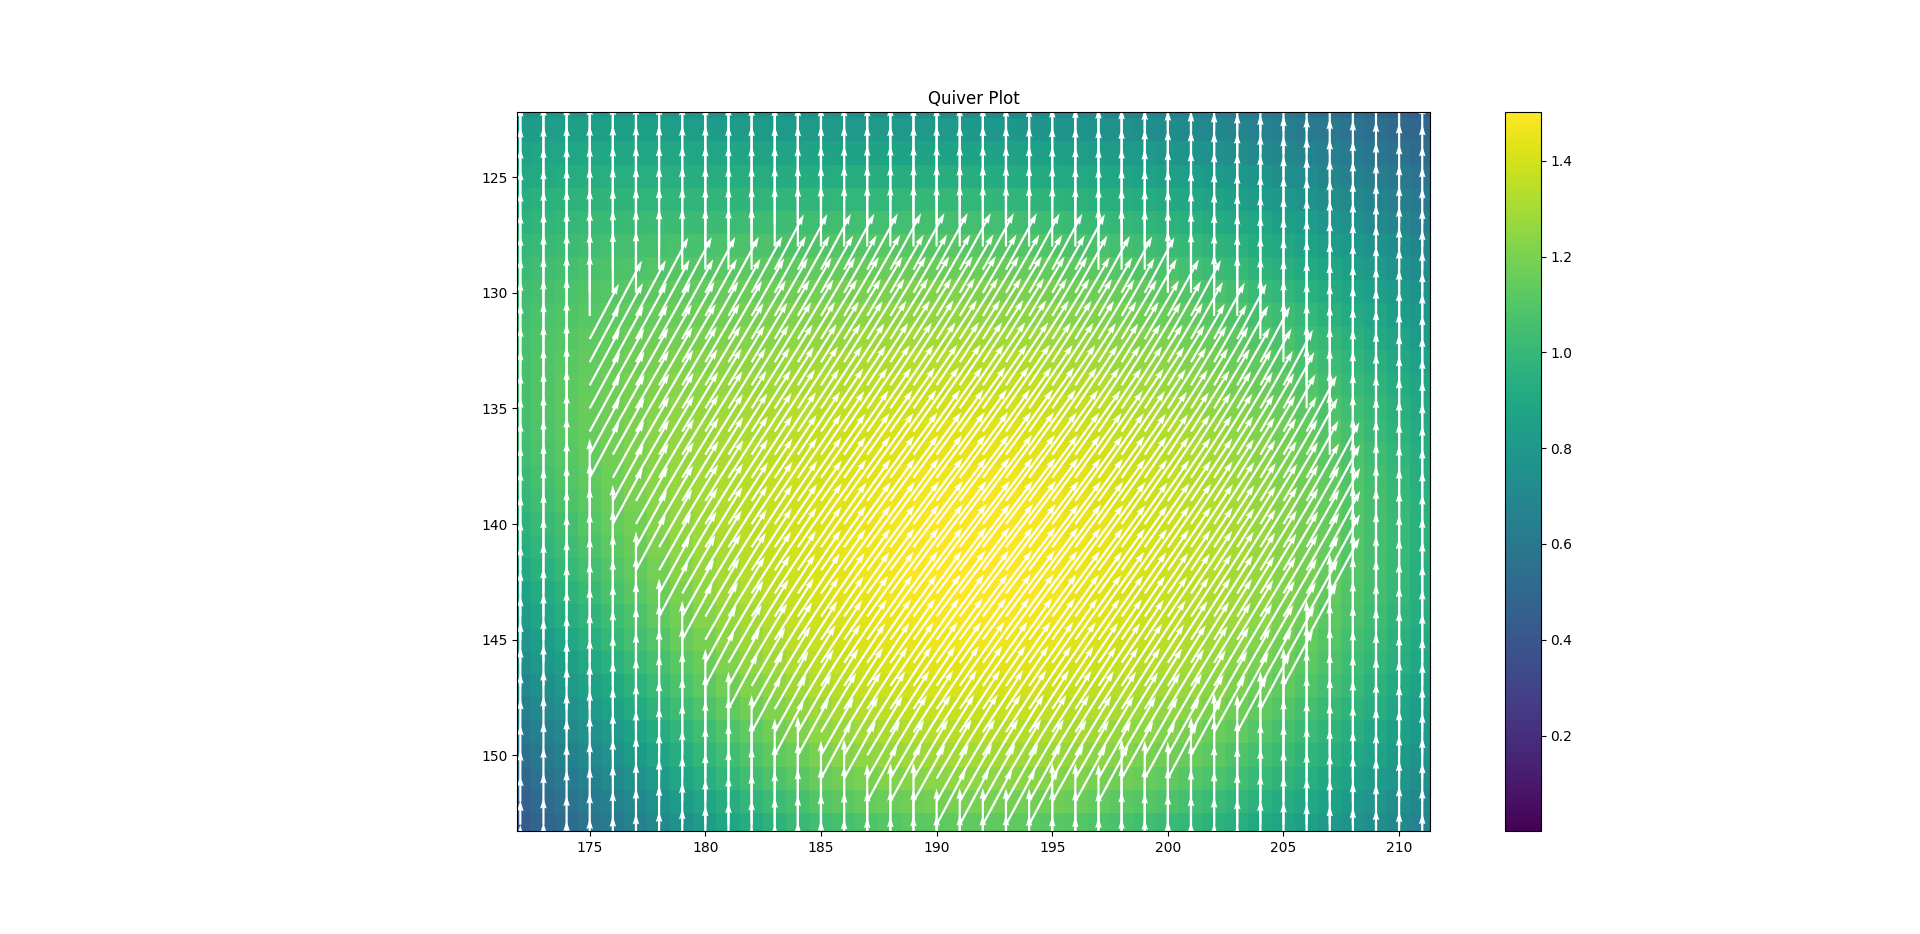
\includegraphics[width=\linewidth]{../Pictures/preferred_1_zoom2.png}
	\end{minipage}
\end{frame}
\end{document}
